\newpage
\section{Diseño del sistema}
\label{sec:diseno_sistema}

El diseño de un sistema basado en inteligencia ambiental requiere la definición de una arquitectura sólida que articule la adquisición de datos, el transporte de señales y la lógica de conmutación perimetral. En este capítulo se detalla la modelización estructural de la infraestructura, abstrayendo los componentes en capas funcionales. Asimismo, se expone el modelado lógico mediante casos de uso, la topología física de los nodos de hardware, el desarrollo analítico del algoritmo de fusión de sensores y la estructuración de los flujos de información locales.

\subsection{Arquitectura general del sistema}
Para garantizar la modularidad, la mantenibilidad y el aislamiento perimetral exigido por los requisitos no funcionales, se ha diseñado una arquitectura jerárquica dividida en cuatro capas operativas independientes. Esta estructura conceptual abstrae la complejidad del hardware y asegura un acoplamiento débil entre los componentes del sistema \cite{bass2012software}.

\begin{itemize}
    \item \textbf{Capa de adquisición y actuación física:} constituida por los microcontroladores distribuidos (nodos ESP32) y sus respectivos transductores analógicos y digitales (radar FMCW, fotorresistor LDR, sensores climáticos y relés de estado sólido). Su función se limita a la digitalización de variables físicas y a la ejecución inmediata de comandos eléctricos.
    \item \textbf{Capa de transporte y red:} configurada sobre una topolog\'ia en estrella segmentada dentro de la red de \'area local (WLAN). Utiliza el protocolo de transporte TCP/IP sobre enlaces Wi-Fi para dar soporte a la comunicaci\'on bidireccional punto a punto mediante la API nativa de ESPHome. Las conexiones directas de red garantizan el intercambio inmediato de estados e informaci\'on de sensores sin necesidad de intermediarios.
    \item \textbf{Capa de gestión centralizada y lógica contextual:} representa el núcleo computacional del proyecto (motor de contexto), centralizado en la plataforma Home Assistant sobre el servidor perimetral (Raspberry Pi 4). Esta capa unifica las lecturas heterogéneas de la capa física, ejecuta las máquinas de estado y gobierna la proactividad del entorno mediante el disparo de las automatizaciones programadas.
    \item \textbf{Capa de persistencia y aplicación:} encargada del almacenamiento de las series temporales de telemetría en una base de datos local optimizada y de la representación gráfica del estado del sistema a través de una interfaz de usuario centralizada o \textit{dashboard} accesible por el administrador.
\end{itemize}

\begin{figure}[H]
    \centering
    \begin{tikzpicture}[
        layer/.style={
            rectangle,
            draw=Azul!80,
            fill=Azul!10,
            rounded corners=3pt,
            very thick,
            minimum width=12.5cm,
            minimum height=1.1cm,
            align=center,
            font=\bfseries\small
        },
        arrow/.style={
            <->,
            >=stealth,
            very thick,
            draw=Azul!80
        }
    ]
        % Nodes with increased vertical spacing (3.0cm intervals)
        \node[layer, fill=Morado!10, draw=Morado!80] (l4) at (0, 9.0) {Capa de persistencia y aplicación\\{\normalfont\footnotesize (Base de datos de series temporales en memoria y Dashboard de usuario)}};
        \node[layer, fill=Azul!10, draw=Azul!80] (l3) at (0, 6.0) {Capa de gestión centralizada y lógica contextual\\{\normalfont\footnotesize (Motor de contexto, máquina de estados finitos y automatizaciones en Home Assistant)}};
        \node[layer, fill=Verde!10, draw=Verde!80] (l2) at (0, 3.0) {Capa de transporte y red\\{\normalfont\footnotesize (API nativa de ESPHome sobre conexiones TCP en Wi-Fi local)}};
        \node[layer, fill=Naranja!10, draw=Naranja!80] (l1) at (0, 0.0) {Capa de adquisición y actuación física\\{\normalfont\footnotesize (Placas de desarrollo ESP32, fotorresistor LDR, sensor climático, radar mmWave y relés)}};

        % Arrows (with 1.6cm physical gap, preventing overlaps)
        \draw[arrow, draw=Morado!80] (l4.south) -- (l3.north);
        \draw[arrow, draw=Azul!80] (l3.south) -- (l2.north);
        \draw[arrow, draw=Verde!80] (l2.south) -- (l1.north);
    \end{tikzpicture}
    \caption{Arquitectura en capas de la infraestructura domótica local.}
    \label{fig:arquitectura_capas_sistema}
\end{figure}

\subsection{Modelado lógico del sistema}
\label{sec:modelado_logico}
La interacción entre los actores identificados y las funciones principales de la infraestructura se formaliza mediante la definición de los casos de uso esenciales del sistema, detallados a continuación:

\subsubsection{Caso de uso 1: inferencia dinámica de presencia y ocupación}
\begin{itemize}
    \item \textbf{Actor principal:} usuario habitual.
    \item \textbf{Actor secundario:} motor de contexto.
    \item \textbf{Descripción:} el usuario habitual entra, permanece inmóvil o abandona la estancia. El sistema evalúa continuamente las compuertas de distancia del radar FMCW y las fluctuaciones lumínicas para actualizar el estado contextual de la habitación en tiempo real, operando de manera transparente.
\end{itemize}

\subsubsection{Caso de uso 2: control ergonómico proactivo de iluminación}
\begin{itemize}
    \item \textbf{Actor principal:} motor de contexto.
    \item \textbf{Actor secundario:} usuario habitual.
    \item \textbf{Descripción:} al detectarse la transición al estado de \textit{estudio} bajo umbrales de luminosidad natural inferiores a los límites paramétricos establecidos, el sistema conmuta automáticamente el relé principal para activar la iluminación de apoyo, protegiendo la salud visual del usuario sin requerir su intervención.
\end{itemize}

\subsubsection{Caso de uso 3: gestión del bienestar y mitigación del sedentarismo (Pomodoro espacial)}
\begin{itemize}
    \item \textbf{Actor principal:} motor de contexto.
    \item \textbf{Actor secundario:} administrador (vía dispositivo móvil).
    \item \textbf{Descripción:} el sistema monitoriza la persistencia ininterrumpida del estado de \textit{estudio}. Si el temporizador lógico alcanza el umbral de 50 minutos sin alteraciones, el motor de contexto genera un parpadeo cíclico en la iluminación general mediante la alternancia del relé y despacha de forma simultánea una notificación \textit{push} de advertencia ergonómica al terminal del usuario.
\end{itemize}

\subsection{Diseño de la red de hardware}
La red de hardware se compone de tres nodos empotrados independientes basados en el soc ESP32, cuya selección responde a su capacidad de cómputo, conectividad Wi-Fi nativa y versatilidad de interfaces GPIO para la adquisición paralela de señales analógicas y digitales.

\subsubsection{Nodo 1: monitorización macroambiental y actuación (nodo ambiente)}
Este nodo se ubica en el perímetro general de la estancia y asume las tareas de adquisición climática, lumínica, acústica y conmutación de potencia. Su arquitectura de hardware integra los siguientes componentes:
\begin{itemize}
    \item \textbf{Gestión lumínica:} un fotorresistor (LDR) acoplado a un circuito divisor de tensión que transforma las variaciones de resistencia óhmica en una señal de tensión analógica, mapeada continuamente por el convertidor analógico-digital (ADC) del microcontrolador.
    \item \textbf{Actuación de potencia:} un módulo de relé de estado sólido con aislamiento galvánico mediante optoacopladores, conectado a un pin GPIO configurado como salida digital, encargado de interrumpir o habilitar el paso de corriente alterna hacia la luminaria principal de la estancia.
    \item \textbf{Telemetría termo-higrométrica:} un transductor digital de temperatura y humedad relativa, conectado mediante un bus serie unifilar (\textit{single-wire}), que suministra lecturas calibradas periódicas para evaluar las condiciones de habitabilidad de la estancia.
    \item \textbf{Monitoreo acústico:} un sensor de sonido de alta sensibilidad (\textit{big sound}), equipado con un micrófono de electret y un comparador analógico basado en el circuito integrado LM393. Este dispositivo se conecta a interfaces digitales y analógicas del ESP32, permitiendo capturar picos de presión acústica ambientales para la inferencia de estados conductuales o la activación de alertas de intrusión.
\end{itemize}

\begin{figure}[H]
    \centering
    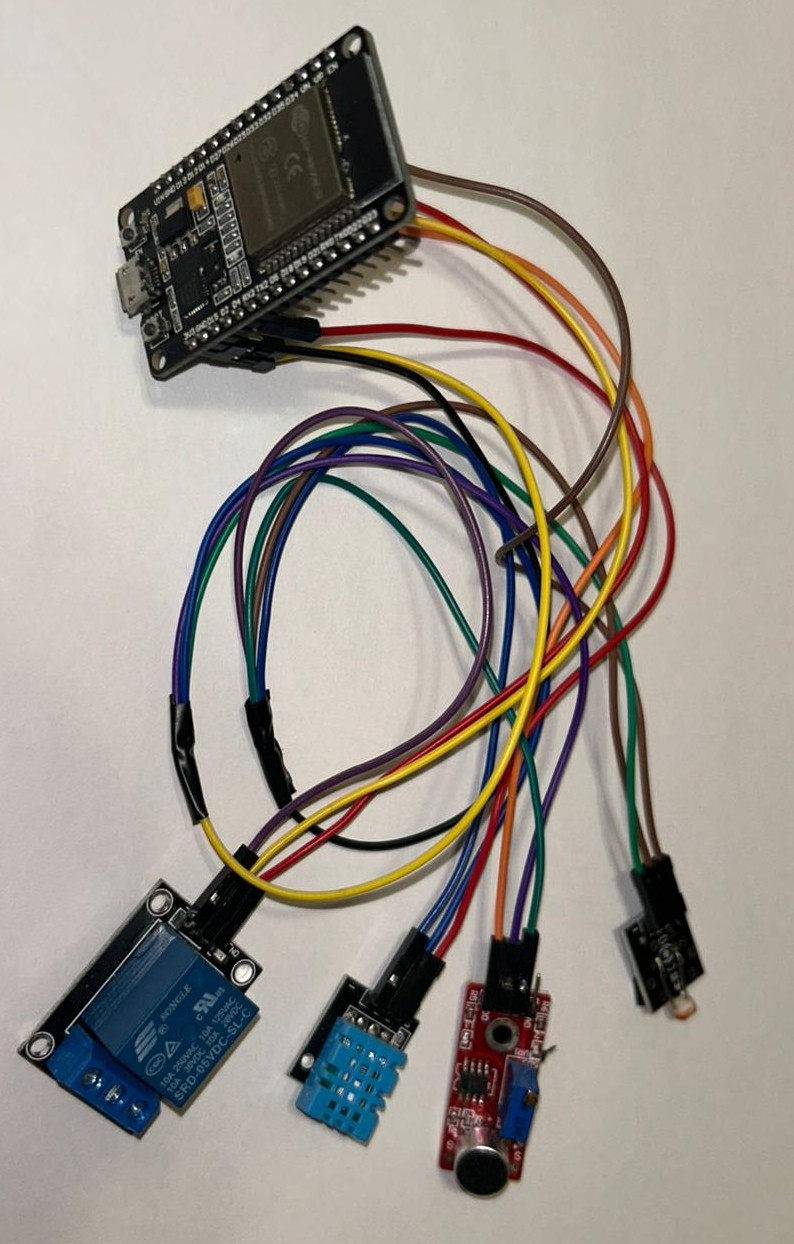
\includegraphics[width=0.7\textwidth]{Img/nodo_ambiente.jpg}
    \caption{Prototipo físico y conexionado de componentes del Nodo 1 (Nodo Ambiente).}
    \label{fig:foto_nodo1}
\end{figure}

\subsubsection{Nodo 2: telemetría espacial y disuasión óptica (nodo escritorio)}
Situado de forma estratégica en el área de trabajo para garantizar la cobertura directa del plano del usuario, este nodo asume las tareas de detección biométrica volumétrica y señalización perimetral mediante la integración de dos subsistemas principales:
\begin{itemize}
    \item \textbf{Transductor volumétrico:} el radar de ondas milimétricas HLK-LD2410C, interconectado con el soc ESP32 a través de un bus de comunicación serie UART (\textit{universal asynchronous receiver-transmitter}) empleando los pines dedicados de transmisión (TX) y recepción (RX). Esta interfaz de alta velocidad permite extraer de manera síncrona los vectores de energía y distancia correspondientes a objetivos dinámicos y estacionarios.
    \item \textbf{Emisor óptico:} un módulo de diodo láser semiconductor conectado a un pin GPIO configurado como salida digital. Este componente actúa como un dispositivo indicador físico de estado y disuasión perimetral, gobernado por el motor algorítmico durante el armado del sistema de alarma o como señal de advertencia secundaria en los ciclos lógicos de trabajo.
\end{itemize}

\begin{figure}[H]
    \centering
    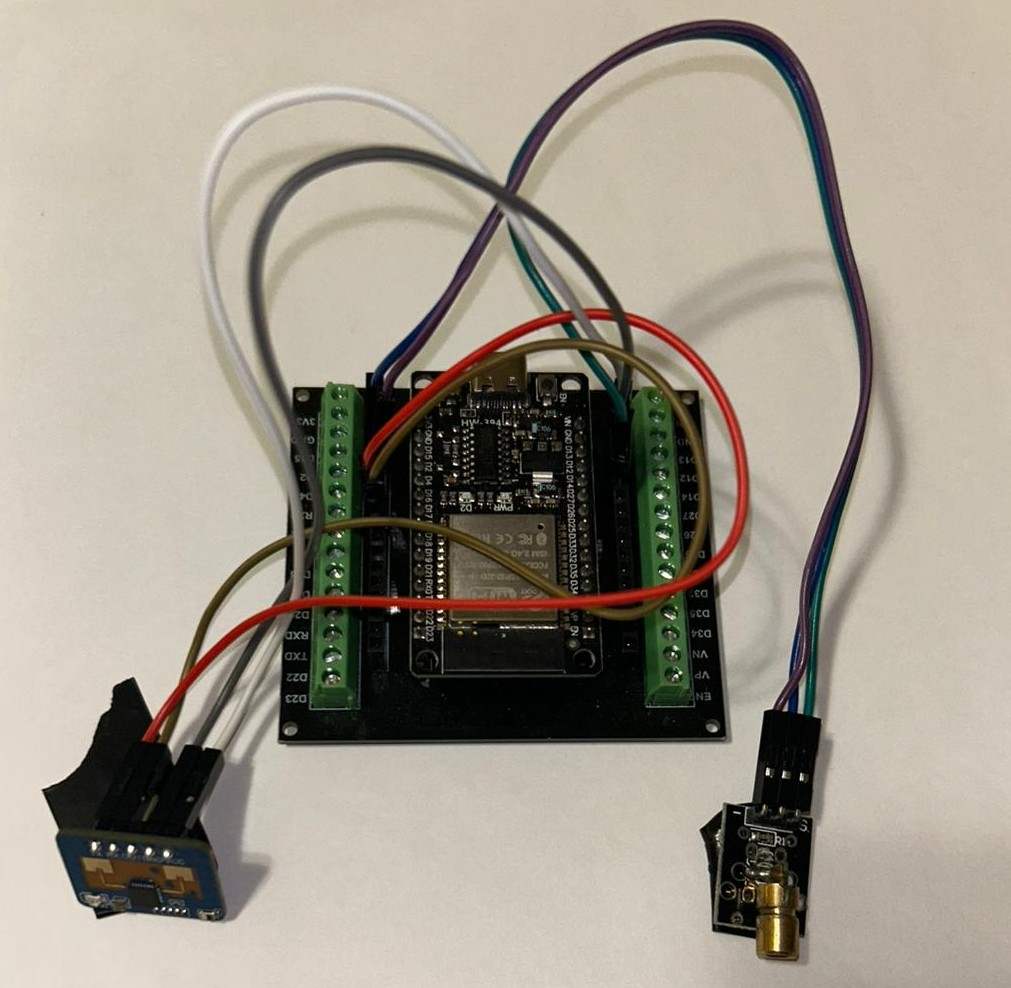
\includegraphics[width=0.7\textwidth]{Img/nodo_escritorio.jpg}
    \caption{Prototipo físico y conexionado de componentes del Nodo 2 (Nodo Escritorio).}
    \label{fig:foto_nodo2}
\end{figure}

\subsubsection{Nodo 3: seguridad perimetral y control de acceso (nodo puerta)}
Ubicado de forma fija en el acceso principal de la estancia, este nodo asume la función exclusiva de supervisar la integridad perimetral del espacio para nutrir el subsistema de alarma. Integra un transductor de contacto magnético de tipo interruptor reed, cuyo funcionamiento se basa en la conmutación eléctrica ante la proximidad de un campo magnético solidario a la hoja de la puerta. El sensor se conecta directamente a un pin GPIO configurado como entrada digital con resistencia de polarización activa (\textit{pull-up}). Las transiciones de estado físico abren o cierran el circuito, disparando interrupciones por hardware en el microcontrolador para garantizar el registro inmediato del evento y mitigar los retardos asociados al muestreo por sondeo (\textit{polling}), transmitiendo la condición de apertura o cierre de forma instantánea hacia el agente de comunicaciones.

\begin{figure}[H]
    \centering
    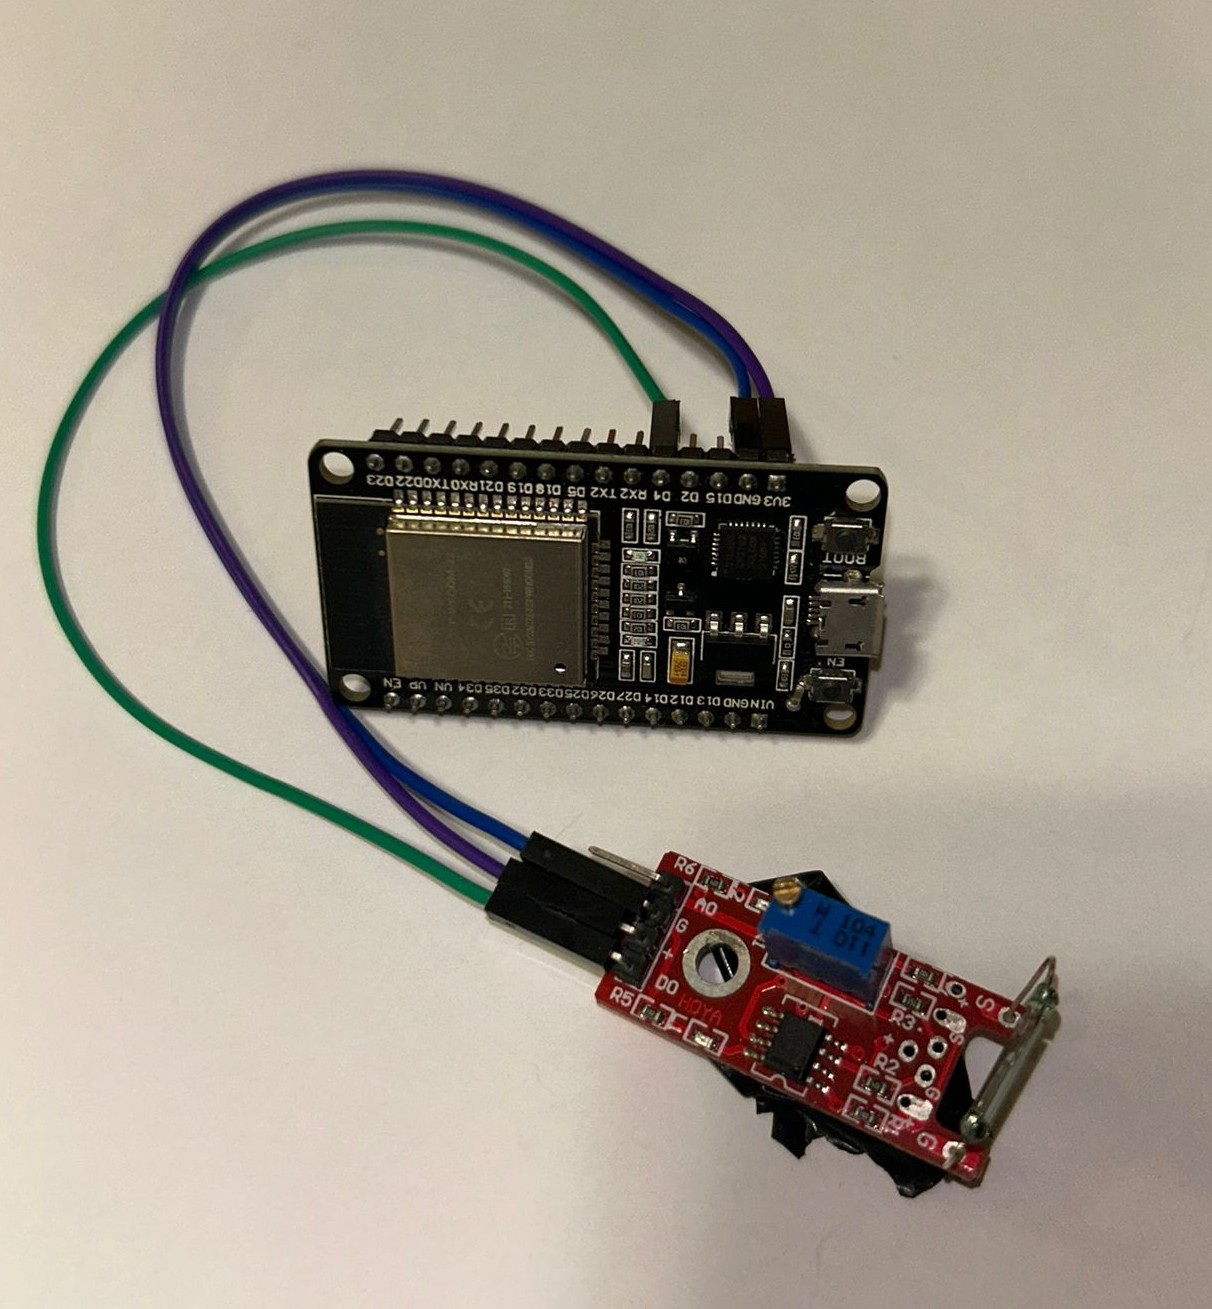
\includegraphics[width=0.7\textwidth]{Img/nodo_puerta.jpg}
    \caption{Prototipo físico e instalación del interruptor magnético del Nodo 3 (Nodo Puerta).}
    \label{fig:foto_nodo3}
\end{figure}

\subsection{Diseño del algoritmo de fusión de sensores (motor de contexto)}
El comportamiento adaptativo del sistema se gobierna mediante una máquina de estados finitos (FSM, por sus siglas en inglés) que ejecuta la fusión de datos en el extremo (\textit{edge}). El sistema abstrae la situación del entorno en cuatro estados discretos estables: \textbf{ausente}, \textbf{ocio}, \textbf{estudio} y \textbf{durmiendo}.

La transición entre estados no depende de un único sensor aislado, sino del procesamiento condicional cruzado de la telemetría entrante, aplicando redundancia lógica para garantizar la tolerancia a fallos. El modelo matemático de transiciones se rige por las siguientes reglas de inferencia:

\begin{equation}
\text{Transición a estudio: } \{ P_{\text{mmWave}} = 1 \} \land \{ D_{\text{objetivo}} \le R_{\text{escritorio}} \} \land \{ T_{\text{estudio}} \ge t_{\text{filtro}} \}
\end{equation}

Donde $P_{\text{mmWave}}$ representa la presencia detectada por el radar, $D_{\text{objetivo}}$ es la distancia cuantitativa registrada y $R_{\text{escritorio}}$ delimita el radio físico del área de trabajo. Un temporizador de seguridad ($t_{\text{filtro}}$) evita falsas transiciones por cruces esporádicos.

Para solventar contingencias críticas de hardware (como la degradación o fallo de lectura de un sensor individual), el algoritmo incorpora bucles de redundancia y reseteo activo. Si el sistema se encuentra en estado \textbf{durmiendo} debido a una lectura baja fija del LDR provocada por un fallo eléctrico, pero el canal analógico del radar computa una ausencia prolongada ($P_{\text{mmWave}} = 0$) durante un tiempo continuo $t_{\text{ausencia}} \ge 20 \text{ minutos}$, el motor de contexto anula de forma proactiva la prioridad del sensor lumínico, forzando la transición segura al estado \textbf{ausente} y mitigando el congelamiento lógico de la infraestructura.

\begin{figure}[H]
    \centering
    \begin{tikzpicture}[
        state/.style={
            circle,
            draw=Azul!80,
            fill=Azul!10,
            very thick,
            minimum size=2.4cm,
            align=center,
            font=\bfseries\small
        },
        trans/.style={
            ->,
            >=stealth,
            thick,
            draw=gray!80,
            align=center,
            font=\scriptsize
        }
    ]
        % Nodes with increased spacing (7.5cm horizontal, 5.0cm vertical)
        \node[state, fill=Rojo!10, draw=Rojo!80] (ausente) at (0, 5.0) {Ausente};
        \node[state, fill=Naranja!10, draw=Naranja!80] (ocio) at (7.5, 5.0) {Ocio};
        \node[state, fill=Verde!10, draw=Verde!80] (estudio) at (7.5, 0.0) {Estudio};
        \node[state, fill=Morado!10, draw=Morado!80] (durmiendo) at (0, 0.0) {Durmiendo};

        % Transitions with clean bend curves and wrapped labels
        \path (ausente) edge[trans, bend left=20] node[above, midway] {Presencia\\($P_{\text{mmWave}} = 1$)} (ocio);
        \path (ocio) edge[trans, bend left=20] node[below, midway] {Ausencia\\($P_{\text{mmWave}} = 0$)} (ausente);
        
        \path (ocio) edge[trans, bend left=20] node[right, midway] {En escritorio y\\$T_{\text{estudio}} \ge t_{\text{filtro}}$} (estudio);
        \path (estudio) edge[trans, bend left=20] node[left, midway] {Fuera de\\escritorio} (ocio);
        
        \path (estudio) edge[trans, bend left=20] node[below, midway] {Luz LDR $\le$ umbral\\y reposo} (durmiendo);
        \path (durmiendo) edge[trans, bend left=20] node[above, midway] {Presencia o\\movimiento} (estudio);
        
        \path (durmiendo) edge[trans, bend left=20] node[left, midway] {Ausencia\\$\ge 20$ min\\(redundancia)} (ausente);
        \path (ausente) edge[trans, bend left=20] node[right, midway] {Modo noche\\y reposo} (durmiendo);
    \end{tikzpicture}
    \caption{Diagrama de la Máquina de Estados Finitos (FSM) para la inferencia de estados contextuales.}
    \label{fig:fsm_estados}
\end{figure}

\subsection{Diseño de la base de datos y flujos de información}
El flujo de información sigue un modelo síncrono y bidireccional basado en la API nativa de ESPHome \cite{al2015internet}. Los nodos sensores operan de forma autónoma, digitalizando las variables térmicas, lumínicas y espaciales a una frecuencia de muestreo parametrizada. Cada lectura actualiza una entidad expuesta en el servidor a través de sockets TCP directos en el puerto 6053, sin necesidad de parsear tramas de texto complejas ni depender de brokers de mensajería intermedios.

El servidor central central captura las actualizaciones de estado de manera inmediata. Al recibir un nuevo evento, se despierta el hilo de ejecución del motor de contexto, que evalúa las condiciones de la FSM. Si se determina un cambio de estado, se genera un evento interno en el bus de Home Assistant que dispara dos acciones concurrentes:
\begin{enumerate}
    \item \textbf{Actuación perimetral:} se invoca el servicio de conmutación correspondiente de vuelta hacia el nodo ESP32 a través del canal abierto de la API, forzando la activación física del relé.
    \item \textbf{Persistencia temporal:} el estado indexado y la telemetría asociada se envían al subsistema de almacenamiento local. La base de datos, estructurada como un motor de series temporales de ejecución en memoria con volcado cíclico al almacenamiento secundario local, registra la tupla compuesta por el identificador de la entidad, el valor transformado y la marca de tiempo precisa (\textit{timestamp}) proporcionada por el sistema operativo del servidor. Esto permite la auditoría posterior de las rutinas del usuario sin comprometer datos fuera de la red local.
\end{enumerate}

\begin{figure}[H]
    \centering
    \begin{tikzpicture}[
        block/.style={
            rectangle,
            draw=Azul!80,
            fill=Azul!10,
            rounded corners=2pt,
            thick,
            minimum width=3.2cm,
            minimum height=1.1cm,
            align=center,
            font=\bfseries\footnotesize
        },
        arrow/.style={
            ->,
            >=stealth,
            thick,
            draw=gray!80
        },
        txt/.style={
            align=center,
            font=\scriptsize\itshape
        }
    ]
        % Nodes
        \node[block, fill=Naranja!10, draw=Naranja!80] (sensores) at (-4.0, 1.5) {Nodos de Control\\(ESP32)};
        \node[block, fill=Azul!10, draw=Azul!80] (ha) at (4.0, 1.5) {Servidor central\\(Home Assistant)};
        \node[block, fill=Morado!10, draw=Morado!80] (db) at (4.0, -1.8) {Persistencia\\(Base de Datos)};
        \node[block, fill=Rojo!10, draw=Rojo!80] (rele) at (-4.0, -1.8) {Actuador\\(Módulo Relé)};

        % Paths
        \draw[arrow] (sensores) to[bend left=20] node[above, txt] {1. Actualiza estado\\(Socket TCP / ProtoBuf)} (ha);
        \draw[arrow] (ha) to[bend left=20] node[below, txt] {2. Ordena conmutación\\(API nativa ESPHome)} (sensores);
        \draw[arrow] (ha) -- node[right, txt] {3. Registra\\series\\temporales} (db);
        \draw[arrow] (sensores) -- node[left, txt] {4. Conmutación\\física (GPIO)} (rele);
    \end{tikzpicture}
    \caption{Diagrama de flujos de información e integración mediante la API nativa de ESPHome en la red local.}
    \label{fig:flujo_informacion}
\end{figure}

\subsection{Análisis de frecuencias y coexistencia (banda ISM)}
Tanto la red troncal Wi-Fi como la red sensórica secundaria operan en la banda ISM de 2.4 GHz. Para evitar interferencias y pérdida de paquetes, se implementa una estrategia de coexistencia de espectro:
\begin{itemize}
    \item \textbf{Capa WLAN:} se configura de forma estática en uno de los tres canales no superpuestos (1, 6 u 11) con un ancho de banda de 20 MHz.
    \item \textbf{Capa WPAN (BLE):} utiliza los canales 37, 38 y 39 en exclusiva para las tramas pasivas (\textit{advertising}) de los sensores. Estos canales se sitúan en los extremos y huecos de la banda, esquivando las frecuencias centrales Wi-Fi. Para las comunicaciones activas, se emplea el algoritmo AFH (\textit{Adaptive Frequency Hopping}) para esquivar el espectro saturado por la WLAN.
\end{itemize}

\subsection{Protocolos de comunicación y modelo OSI}
El flujo de información atraviesa dos pilas de protocolos distintas. Las placas ESP32 actúan como pasarelas de aplicación (\textit{application layer gateways}) para unificar el entorno perimetral:

\begin{table}[H]
    \centering
    \setlength{\tabcolsep}{4pt}
    \renewcommand{\arraystretch}{1.2}
    \begin{tabular}{|c|c|c|}
        \hhline{|-|-|-|}
        \rowcolor[gray]{0.9} 
        \parbox[c]{3.5cm}{\vspace{0.2cm}\centering\textbf{Capa OSI}\vspace{0.2cm}} & \parbox[c]{5.25cm}{\vspace{0.2cm}\centering\textbf{Red sensórica (WPAN)}\vspace{0.2cm}} & \parbox[c]{5.25cm}{\vspace{0.2cm}\centering\textbf{Red troncal (WLAN)}\vspace{0.2cm}} \\ \hhline{|-|-|-|}
        \parbox[c]{3.5cm}{\vspace{0.2cm}\centering\textbf{7. Aplicación}\vspace{0.2cm}} & \parbox[c]{5.25cm}{\vspace{0.2cm}\centering Perfiles GAP / GATT (tramas \textit{advertising})\vspace{0.2cm}} & \parbox[c]{5.25cm}{\vspace{0.2cm}\centering API nativa ESPHome\vspace{0.2cm}} \\ \hhline{|-|-|-|}
        \parbox[c]{3.5cm}{\vspace{0.2cm}\centering\textbf{6. Presentación}\vspace{0.2cm}} & \parbox[c]{5.25cm}{\vspace{0.2cm}\centering Integrado en capa 7\vspace{0.2cm}} & \parbox[c]{5.25cm}{\vspace{0.2cm}\centering Protocol Buffers (binario)\vspace{0.2cm}} \\ \hhline{|-|-|-|}
        \parbox[c]{3.5cm}{\vspace{0.2cm}\centering\textbf{5. Sesión}\vspace{0.2cm}} & \parbox[c]{5.25cm}{\vspace{0.2cm}\centering Sin conexión (\textit{connectionless})\vspace{0.2cm}} & \parbox[c]{5.25cm}{\vspace{0.2cm}\centering Sockets TCP persistentes\vspace{0.2cm}} \\ \hhline{|-|-|-|}
        \parbox[c]{3.5cm}{\vspace{0.2cm}\centering\textbf{4. Transporte}\vspace{0.2cm}} & \parbox[c]{5.25cm}{\vspace{0.2cm}\centering No aplica en topología pasiva\vspace{0.2cm}} & \parbox[c]{5.25cm}{\vspace{0.2cm}\centering TCP (con control de flujo)\vspace{0.2cm}} \\ \hhline{|-|-|-|}
        \parbox[c]{3.5cm}{\vspace{0.2cm}\centering\textbf{3. Red}\vspace{0.2cm}} & \parbox[c]{5.25cm}{\vspace{0.2cm}\centering No aplica en topología punto a punto\vspace{0.2cm}} & \parbox[c]{5.25cm}{\vspace{0.2cm}\centering IPv4 (Enrutamiento local)\vspace{0.2cm}} \\ \hhline{|-|-|-|}
        \parbox[c]{3.5cm}{\vspace{0.2cm}\centering\textbf{1 y 2. Física / Enlace}\vspace{0.2cm}} & \parbox[c]{5.25cm}{\vspace{0.2cm}\centering Direccionamiento MAC BLE. Modulación GFSK (banda 2.4 GHz).\vspace{0.2cm}} & \parbox[c]{5.25cm}{\vspace{0.2cm}\centering Direccionamiento MAC Wi-Fi. IEEE 802.11ax (OFDMA).\vspace{0.2cm}} \\ \hhline{|-|-|-|}
    \end{tabular}
    \caption{Pila de protocolos y mapeo del Modelo OSI en la arquitectura de red.}
    \label{tab:protocolos_osi}
\end{table}

\textbf{Mecanismo de consistencia y control de flujo:}
Al operar sobre la API nativa de ESPHome, se prescinde de la capa de sobrecarga de QoS de MQTT. En su lugar, el protocolo de ESPHome emplea sockets TCP persistentes orientados a conexión que garantizan la entrega en orden de todas las tramas de datos. La API implementa un mecanismo de latido activo (\textit{keepalive}) para detectar desconexiones en un plazo inferior a 5 segundos, y un sistema de cola en memoria local para registrar eventos transitorios y retransmitirlos automáticamente al restablecer el enlace con el servidor central.